\chapter{Estatística univariada}

O primeiro passo para a avaliação de um recurso mineral é descrever as amostras retiradas em campo. O que desejamos nesta etapa é resumir estatisticamente um conjunto grande de informações. Uma tabela contendo vários números é de difícil compreensão quando lida, mas ao resumir a informação relatando que 90 por cento dos dados estão acima de um teor de 5g/tonelada, ou que 70 por cento do depósito mineral é constituído do litotipo 1, torna-se mais fácil a tarefa da tomada de decisão. Dados são convertidos em informações quando é possível tomar juízos a partir deles. 

Nete caso estamos interessados em saber se as amostras estão acima de um valor de cut-off prescrito, quais são os valores mínimos e máximos, se suas variações são pequenas ou grandes, quais são os valores mais comuns e incomuns. Todas essas informações são necessárias para que um engenheiro ou geólogo possa resolver problemas em uma mina. 

Imaginem que um avaliador tenha em mãos os dados de testemunhos de sondagem regularmente espaçados ao longo de uma área, com um valor de teor médio de $5.2\%$ e um desvio padrão de $2\%$. Ou seja, há uma grande chance de que os valores de teor da área estejam entre $7.2\%$ e $3.2\%$. Para aquele depósito mineral, o avaliador sabe que o cut-off para o depósito é de $12\%$. Dessa forma as chances daquela área se tornar um recurso são ínfimas. Ele pode recusar a campanha de exploração se não houverem recursos para continuá-la. Os dados se transformaram em uma informação a partir das estatísticas e com ela pôde-se tomar uma decisão sobre o empreendimento.  

É importante entender que toda a estatística transforma dados em informação, mas em contrapartida perde a sensibilidade dos valores das amostras. A média e o desvio padrão são funções que resumem os dados, mas deixam de ressaltar peculiaridades inerentes da distribuição dos dados.

Tomemos como exemplo dois blocos dentro de uma mina. Digamos que um seja um minério com alto valor agregado, e outro um estéril muito pobre. Digamos que a média dos seus valores ainda seja considerada minério, tal como mostrado na figura \ref{Fig9_1}. Se lavrarmos dois blocos conjuntamente temos ainda um grande bloco de minério, pois sabemos que seu valor médio está acima do limite econômico, no entanto, perdemos a sensibilidade dos dados pois sabemos que há um valor que poderia ser recusado como um estéril.

\begin{figure}[H]
\centering
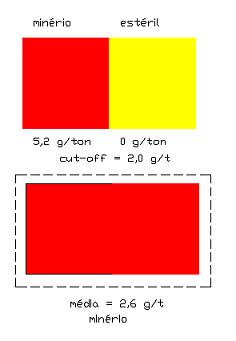
\includegraphics[scale=1]{figura9_1.png}	
\caption{Média de dois blocos - Um estéril e outro 
	minério. Os dois blocos são considerados conjuntamente como minério se tomarmos o valor médio }
\label{Fig9_1}
\end{figure}

Esta falta de sensibilidade dos dados, que as estatísticas causam, faz com que seja necessário incorporar mais funções na análise para entendermos as propriedades dos dados. É inadmissível caracterizarmos um depósito apenas situando seus valores médios. É sempre importante agregarmos o máximo de informação possível. 

\section{Valores outliers}

A primeira etapa da geoestatística é a validação das amostras. Devemos antes de tudo verificá-las para que não encontremos valores discrepantes (outliers) ou incoerências nos dados. Além disso, a estatística descritiva é responsável por determinar as primeiras informações a respeito do depósito mineral. Esta é uma etapa necessária antes que se prossigam com os métodos geoestatísticos. É obrigação do avaliador de reservas verificar se as metodologias de amostragem e os valores inseridos no banco de dados estão corretos. A Tabela \ref{Tabela1:Minerio_de_ferro} é um exemplo de como valores anômalos podem aparecer. Nota-se claramente que as amostras 1 e 3 estão erradas. Primeiramente porque não existem valores de teor percentuais acima de 100$\%$ e também porque não existem teores descritos como letras. No entanto, a amostra 4 também está errada, porque o minério composto por limonita não pode apresentar um valor de teor de ferro de 72$\%$, pois é incompatível com a  química da mineralogia. 


\begin{table}[H]
\centering
\caption{Tabela de teores do minerio de ferro}
\vspace{0.5cm}
\label{Tabela1:Minerio_de_ferro}
\begin{tabular}{r|lr}
	
	Índice & Minério & Teor($\%$) \\ 
	\hline                               
	1 & Hematita compacta       & 120$\%$ \\
	2 & Hematita granular       & 53$\%$ \\
	3 & Magnetito               & 0.i3 \\
	4 & Limonita                & 72$\%$ \\

\end{tabular}
\end{table}

Um gráfico que auxilia para determinar valores outliers é chamado de boxplot. Ele demonstra a disposição dos dados em um eixo e limita os valores das amostras em uma caixa contendo os quartis das amostras. Os valores que se situam acima ou abaixo de 1.5 do intervalo interquartil representam outliers. O intervalo interquartil é também determinado como a diferença entre os valores do terceiro quartil e do primeiro quartil. A figura \ref{fig7_1} demonstra o gráfico boxplot e suas dimensões. 

\begin{figure}[H]
\centering
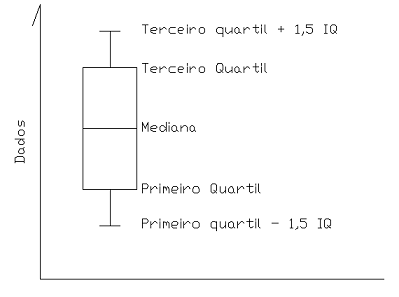
\includegraphics[scale=0.80]{figura7_1.png}	
\caption{Representação de um gráfico de caixa dividida entre os intervalos das amostras }
\label{fig7_1}
\end{figure}

Os valores anômalos ou outliers são demonstrados na figura \ref{Fig8_1} como pontos circulados fora das barras que representam os limites de aceitação dos valores da amostra.

\begin{figure}[H]
	\centering
	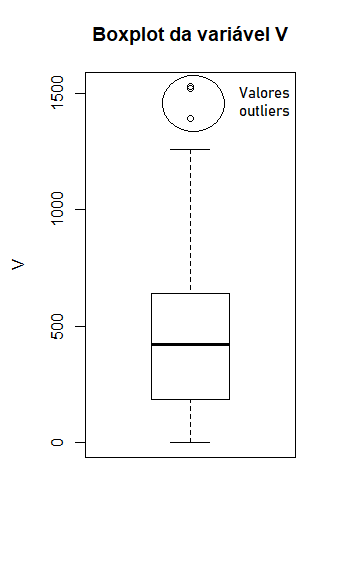
\includegraphics[scale=0.90]{figura8_1.png}	
	\caption{Representação dos valores outliers no gráfico boxplot - Pontos circulados em vermelho }
	\label{Fig8_1}
\end{figure}


 É importante entender que os dados anômalos nem sempre são valores errados. Eles podem ser valores reais representantes de uma anomalia da natureza. Poderíamos encontrar, por exemplo, em um depósito de ouro uma pepita com um valor agregado muito alto, mas apesar de ser um dado correto ele não representa o conjunto de amostras como um todo.

O tratamento de dados discrepantes ou outliers pode ser realizado de diversas maneiras.

\begin{itemize}
	
\item Podemos retirar os dados da avaliação. Esta exclusão deve ser criteriosa e se basear na  qualidade da amostra, na recuperação do testemunho de sondagem ou em um critério definido. A amostragem é a etapa mais cara no processo de avaliação de reservas e por isso a retirada de valores outliers não pode ser realizada como uma rotina.

\item Podemos ponderar o valor da amostra durante a análise. Se um valor outlier representar um dado discrepante em meio a um conjunto de amostras com baixo valor, podemos reduzir sua influência ponderando as estatísticas pela sua área de influência.

\item Podemos tratar a amostra como uma classe separada das outras amostras. Diferenciando as amostras outliers do resto podemos indicar regiões que apresentam propriedades estatísticas diferentes. 
\end{itemize}

É importante salientar que qualquer método de estimativa não cria informação. Se os dados descritivos de uma análise inicial do depósito mineral não indicarem recursos adequados a estimativa constatará da mesma forma a informação. 

Qualquer método de inferência não extrapola os valores mínimos e máximos de um depósito mineral. Descrever é antes de tudo um passo que necessita encontrar propriedades de algo. A descrição deve conter os aspectos mais importantes de um depósito mineral, tal como mínimo e máximo encontrados, valores médios, dispersão. Da mesma forma que desenhar é uma atividade altamente explicativa para descrever um problema, as estatísticas gráficas desempenham papel fundamental na avaliação inicial.

\section{ Descrição espacial das amostras}

O primeiro passo para a descrição espacial é verificar a disposição geométrica das amostras. A figura \ref{Fig1_1} demonstra um depósito polimetálico de Jura. O atributo é o tipo de rocha de um dado período geológico.  

\begin{figure}[H]
\centering
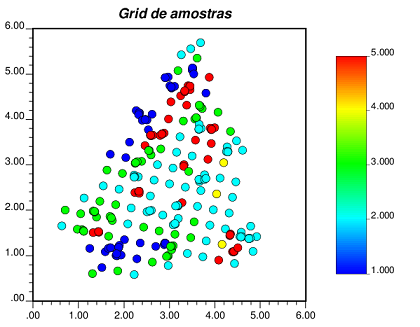
\includegraphics[scale=1]{figura1_1.png}	
\caption{Disposição das amostras no espaço. Cores diferenciadas mostrando tipos de rocha em períodos geológicos diferentes}
\label{Fig1_1}
\end{figure}

Podemos ver que as amostras estão dispostas de forma irregular em um formato de delta de um rio. A orientação do tipo de rocha 1 se encontra ao oeste e parte ao sul, enquanto a do tipo 5 se encontra distribuído mais ao norte. Qualquer estimativa realizada a partir desta configuração de amostras deve respeitar os valores iniciais. Se por exemplo, iniciássemos uma explotação cujo o interesse seria o litotipo 1, provalvelmente começaríamos a retirar o material de oeste para leste para reduzir o fluxo de caixa do empreendimento. 

A \ref{Fig2_1} demonstra o atributo Cádmio acerca deste depósito. Note que o depósito é bem homogêneo quanto a distribuição do elemento. 

\begin{figure}[H]
\centering
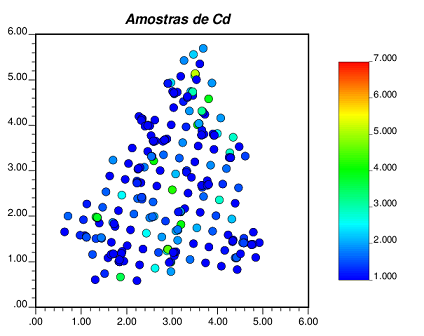
\includegraphics[scale=1]{figura2_1.png}	
\caption{Disposição do Cd}
\label{Fig2_1}
\end{figure}

As informações espaciais das amostras garantem alternativas para associar as variáveis com suas componentes genéticas e interpretar seus valores segundo objetivos desejados. Notamos que o litotipo 1 parece ter maior correlação com valores baixos do teor de Cádmio do que o litotipo 2, que parece ter correlação com valores um pouco mais altos. O primeiro passo da análise visual é verificar regiões de risco, de valores mais ricos ou pobres e identificar padrões de continuidade nas amostras.  

\section{Histograma}

A descrição das estatísticas das amostras é uma forma inicial para aglomerar um conjunto de informações extensos. Um gráfico de grande utilidade para verificar a frequência dos dados é o histograma. Este é uma figura de barras em que a altura de cada retângulo representa a frequência de uma classe.

 A \ref{Fig3_1} representa um histograma da variável Cádmio do depósito de Jura.  

\begin{spacing}{1.0}
\begin{figure}[H]
\centering
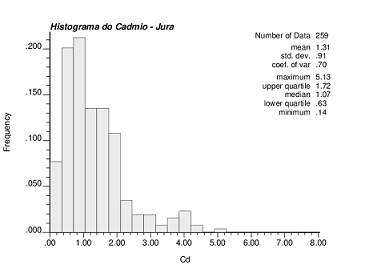
\includegraphics[scale=1]{figura3_1.png}	
\caption{Histograma do Cd}
\label{Fig3_1}
\end{figure}
\end{spacing}

Na \ref{Fig4_1} podemos ver que a classe de teores de $0,04$ a $0,75g/ton$ ocupa uma proporção de 20 \% dos dados.


\begin{figure}[H]
\centering
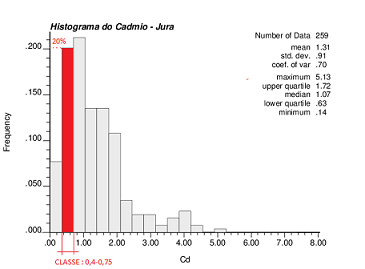
\includegraphics[scale=1]{figura4_1.png}	
\caption{Histograma do Cd - Classe marcada}
\label{Fig4_1}
\end{figure}


Ao contrário da análise espacial, no histograma estamos apenas interessados em determinar o conjunto de informações das amostras. Perdemos a noção de suporte quando utilizamos esta estatística, porém ganhamos recurso para o entendimento valores das amostras. 

Outra forma de representar um histograma é na sua forma acumulada. A figura \ref{Fig5_1} é uma demonstração do gráfico acumulado. 

\begin{figure}[H]
%\centering
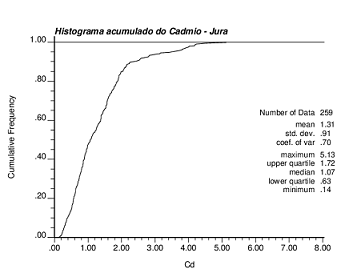
\includegraphics[scale=1]{figura5_1.png}	
\caption{Histograma do Cd acumulado}
\label{Fig5_1}
\end{figure}

A figura \ref{Fig6_1} demonstra a leitura do gráfico acumulado.Podemos notar por este gráfico que 60 por cento dos valores estão abaixo do teor de $1,5 g/tonelada$.  

\begin{figure}[H]
	%\centering
	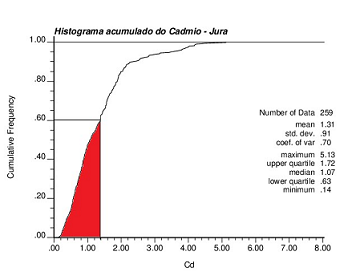
\includegraphics[scale=1]{figura6_1.png}	
	\caption{Histograma do Cd acumulado - Leitura}
	\label{Fig6_1}
\end{figure}



O formato do histograma também é um importante parâmetro para a inferência de distribuições de probabilidade. A partir dele podemos visualizar uma possível distribuição de probabilidade e dar um "chute" para testarmos se esta se encaixa na distribuição das amostras. 

É importante para a escolha da resolução do gráfico um número de classes condizentes. Muitas classes farão várias barras terem valores de apenas 1 unidade, enquanto apenas uma classe incorporará todas as amostras. A fórmula de Sturges é uma boa estimativa para o número mínimo de classes para o histograma, mas nada compete com a iniciativa do analista em encontrar a quantidade que mais se adéqua ao problema. É importante que o histograma demonstre claramente o comportamento de simetria da distribuição, dos valores mais frequentes e da dispersão da variável.

 A simetria é uma medida que indica quão próximos estão os valores distribuídos de um conjunto de amostras perto do seu valor médio. O histograma da figura \ref{Fig3_1} demonstra uma distribuição claramente assimétrica em que os valores mais baixos possuem proporções maiores que os valores mais altos. Isso significa que neste depósito a chance de encontrar uma amostra com teor de Cádmio baixa é alta, mas no entanto, ainda é possível encontrar um valor muito mais alto em uma frequência menor. Distribuições simétricas geralmente são mais comportadas. Estimar seus valores e determinar seus parâmetros se torna mais simples, porque elas giram entorno de um valor esperado. Espera-se menos "surpresas" quando uma distribuição é simétrica. 


\section{Estatísticas pontuais}

Outra forma de resumir e descrever os dados é através de estatísticas pontuais. Elas resumem a informação do conjunto de amostras em uma única medida descrevendo-o como um todo. Se fôssemos comparar a descrição pontual com o retrato falado de um criminoso, cada estatística seria apenas uma parte do rosto, a média o nariz e a variância as orelhas, por exemplo. 

Parece um pouco tolo este tipo de descrição, no entanto, as características de um rosto humano são de fácil reconhecimento para qualquer indivíduo. Isso motivou a criação de um tipo de gráfico específico na estatística chamado também de rostos de Chernoff. 

Existem diversas estatísticas pontuais, cada uma medindo uma propriedade das amostras, mas apenas estamos interessados em 4. Medidas de tendência central, medidas de dispersão, medidas de assimetria e de achatamento.

É importante salientar que apenas uma estatística pontual não é uma medida que garante informação completa a respeito de um conjunto de dados.

 Um depósito mineral pode ter valor médio de 50g de ouro por tonelada, enquanto outro tenha 45g de ouro por tonelada, e ainda assim o segundo depósito seja mais rico. 
 
 Isso acontece porque as medidas pontuais de tendência central como a média devem estar sempre associadas com uma medida de dispersão. Se o depósito de 50 g por tonelada possuir uma menor dispersão, e o depósito de 45 g/ton possuir uma maior, para um dado cut-off o depósito de 45g/ton pode ser mais rico.

A Figura \eqref{explicacao} demonstra esta situação graficamente. Notamos que a a distribuição A, apesar de possuir uma média menor que a distribuição B, ainda assim relata um depósito mais rico para o cut-off considerado. 

\begin{figure}[H]
	%\centering
	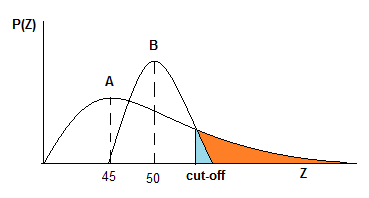
\includegraphics[scale=1]{explicacao1.png}	
	\caption{Exemplo de duas distribuições A e B relatando um depósito mais rico A com média menor que B. Área azul mostrando a contribuição da distribuição B acima do cut-off e área laranja mostrando a contribuição de A acima do cut-off}
	\label{explicacao}
\end{figure}

\subsection{Medidas de tendência central} 

As medidas de tendência central são estatísticas calculadas a partir das amostras que representam o centro de massa do conjunto. Analogamente ao ponto de equilíbrio de uma barra, estas representam o centro de dispersão dos dados. 

Note que esta é uma convenção matemática. O valor médio não representa necessariamente um valor do conjunto de amostras e nem tão pouco pode representar um valor mais provável, mas apenas um centro da dispersão dos dados.

Como exemplo, a média do lançamento de um dado é 3.5 que não constitui nem um valor possível dos dados, nem ao menos o mais provável. Distribuições com histogramas mais simétricos e comportados geralmente podem associar o valor mais provável com a média.  

As medidas de tendência central mais comuns são a média aritimética, a moda, a média ponderada e a mediana. A média aritimética pode ser descrita segundo a equação \eqref{eq3:media aritmetica} em que x são os valores das amostras e n o número de amostras.   

\begin{equation}\label{eq3:media aritmetica}
\bar{x} = \sum_{i = 0}^{n} x_i
\end{equation}

A moda pode ser descrita como o valor mais frequente observado no conjunto de amostras. Nem sempre uma distribuição pode apresentar um valor de moda. Para variáveis contínuas, muitas vezes temos apenas um valor de cada realização. Neste caso não temos moda nenhuma ou todos os valores são a moda e não faz sentido definí-la. 

A média ponderada pode ser descrita pela equação \eqref{eq4: media ponderada}

\begin{equation}\label{eq4: media ponderada}
\bar{x} = \sum_{i = 0}^{n} \lambda_i x_i
\end{equation}

Em que $\lambda_i$ representa o ponderador de cada realização. O ponderador é o valor de cada peso dividido pela soma de pesos totais \eqref{pesos} 
 
\begin{equation}\label{pesos}
\lambda_i = \frac{p_i}{\sum_{i=1}^{n}p_i}
\end{equation}

Logo sabemos que a soma de todos os ponderadores de uma média ponderada é igual a 1 sempre. A média ponderada dos teores é um exemplo em que temos o valor do peso igual ao volume da amostra e o ponderador como a relação de cada volume pelo volume total das amostras. 


\subsection{medidas de posição}

Os quartis são medidas de posição que indicam o valor percentual de uma série ordenada de dados. O primeiro quartil indica o valor ao qual os dados se dividem em 25 por cento de ordem crescente, o segundo quartil também chamado de mediana, divide os dados em 50 por cento e o terceiro quartil em 75 por cento. Outros valores de posição são os percentis, que representam o valor para um percentual acumulado das amostras. 

Se obtivermos um conjunto de dados iguais a ${50,34,27,54,25,43,15,12}$ contendo 8 valores então podemos ordená-los em crescente de tal forma que teremos ${12,15,25,27,34,43,50,54}$. O valor do primeiro quartil será, segundo os dados ordenados, 15. O terceiro quartil será 43. E a mediana será igual a 27. 

\subsection{medidas de dispersão}

Outras medidas importantes são as de dispersão. Entre as mais comuns podemos citar a variância, o desvio padrão e os valores de mínimo e máximo. A variância pode ser descrita pela equação \eqref{eq5:variancia}

\begin{equation}\label{eq5:variancia}
  s^2 = \frac{\sum_{i = 0}^{n} \left( x_i - \bar{x} \right)^2}{n-1}
\end{equation}

Em que n-1 é o número de graus de liberdade da amostra, tal que este pode ser definido pelo número de amostras menos o número de estatísticas utilizadas durante o cálculo. Note que para a operação da variância precisamos antes determinar o valor da média. É uma medida que não apresenta as mesmas unidades que a das amostras, para isso geralmente utilizamos o desvio padrão, que pode ser calculado como a raiz quadrada dos valores da variância. 

\subsection{Conjugando estatísticas pontuais}

Como dito anteriormente, é sempre importante conjugar estatísticas pontuais diferentes de forma a garantir a melhor informação possível. Uma destas alternativas é adicionar ao valor médio um número de desvios padrões de forma a garantir que um conjunto de dados esteja situado dentro destes limites. Para isso utilizaremos uma das mais renomadas relações estatísticas.

A desigualdade de Chebyshev é uma identidade que implica em um valor mínimo de probabilidade para que uma realização esteja dentro de um intervalo múltiplo do desvio padrão. Podemos definir a equação \eqref{eq6:Chebyshev} como a desigualdade de Chebyshev.

\begin{equation}\label{eq6:Chebyshev}
P\left(|Z-\mu| \geq k\sigma\right)\leq1/k^2
\end{equation}

Em que Z é o valor da variável aleatória, $\mu$ é o valor da média da população, $\sigma$ é o valor do desvio padrão da população e k é uma constante proporcional. A desigualdade de Chebyshev é independente do valor da distribuição de probabilidades.

 Para um k igual a 2, sabemos que existe uma probabilidade de no mínimo 75 por cento de que o valor da amostra esteja em dois desvios padrões da média.

Podemos caracterizar as amostras então por uma medida de posição e de dispersão conjuntamente. Ao descrever as amostras é bem claro que devemos associar no mínimo dois de seus parâmetros, como por exemplo, dizer que as amostras de teor de ouro possuem valores entre $\left(50 \pm 20 \right) ppm$ em que 20 representaria dois desvios padrões de 10 ppm e 50 ppm seu valor médio.

\subsection{Assimetria}

Outra medida pontual importante também é a assimetria. Esta se caracteriza pela diferença de proporções de uma distribuição de amostras segundo ao redor de seu valor mais frequente. 

A figura \eqref{Fig10_1} demonstra a distribuição de dados assimétrica. O item a) representa uma distribuição assimétrica positiva, enquanto o item b) representa uma distribuição assimétrica negativa. A assimetria positiva é caracterizada por um valor da mediana abaixo do valor médio, enquanto a assimetria negativa se caracteriza por uma alta proporção de valores altos. 


\begin{figure}[H]
 	\centering
 	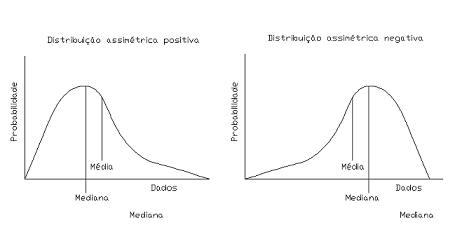
\includegraphics[scale=1.0]{figura10_1.png}	
 	\caption{Assimetria de uma distribuição de dados a) Assimetria positiva b) assimetria negativa }
 	\label{Fig10_1}
\end{figure}

Uma das medidas de assimetria mais comuns é o coeficiente de Pearson que pode ser expresso pela equação \eqref{eq5:coeficiente de pearson}


\begin{equation}\label{eq5:coeficiente de pearson}
\epsilon = \left( \bar{x} - m_0\right)/s
\end{equation}


Em que $m_0$ é a moda dos dados, $\bar{x}$ é o valor médio das amostras e s é o desvio padrão das amostras. 

Distribuições com característica de assimetria positiva são muito comuns na avaliação de depósitos minerais, principalmente no tratamento de commodites erráticos tal como ouro e diamante. Nesses depósitos podem ocorrer anomalias raras e uma amostra constituir em alto valor. Esta propriedade também é chamada de efeito pepita e será melhor tratada no capítulo de Continuidade espacial. 

\subsection{Coeficiente de variação}

Em certos momentos é importante comparar variáveis aleatórias de tipos diferentes. Para sabermos se uma distribuição é mais errática que outra, neste caso, não bastaríamos comparar seus valores de variância. Valores que possuam médias maiores tendem a apresentar dispersões também maiores. Para isso utilizamos o coeficiente de variação, que nada mais é do que o desvio padrão de uma distribuição pelo seu valor médio. Desta forma "igualamos" diferentes distribuições em um único coeficiente comparativo. 

O coeficiente de variação pode ser dado pela equação \eqref{eq5:coeficiente de var}

\begin{equation}\label{eq5:coeficiente de var}
	CV = \frac{s}{\bar{x}}
\end{equation}
 

\section {Inferência Estatística}

Após analisados os dados amostrais podemos utilizar funções para modelar populações dos dados. É importante notar que neste caso estamos definindo uma lei de probabilidade para todo o depósito, independente dos valores locais e ainda não estamos utilizando a geoestatística propriamente. É de pouco interesse para nós modelarmos um depósito mineral sem o conhecimento do suporte dos dados. Logo esta etapa demonstrada aqui, como uma estatística univariada, é muito mais importante a ser realizada depois dos métodos de estimativa ou durante os procedimentos de transformação dos dados. Vamos iniciar alguns tipos de distribuições mais importantes.
,
\subsection{Famílias de distribuições estatísticas}

Uma função de densidade de probabilidade de uma variável aleatória nada mais é do que uma função $p(X = x)$ que correlaciona cada realização da variável aleatória X a uma dada probabilidade. Como consequência da definição algumas condições estão associadas:

\begin{itemize}
	\item $p(x) \leq 1 \forall x$
	\item $\int_{-\infty}^{\infty} p(x) dx = 1$ para distribuições contínuas
	\item $\sum_{x=-\infty}^{\infty} p(x) = 1$ em que a e b são limites para a distribuição discreta
\end{itemize}
 

\subsubsection{Distribuição de Poisson}

Esta é uma distribuição discreta amplamente utilizada para experimentos ditos de eventos "raros", ou seja, utilizada para modelar eventos que a probabilidade de ocorrência é diretamente proporcional ao tempo de espera. 

Em filas de caminhões, por exemplo, é muito comum a utilização da função de distribuição de Poisson para medir a probabilidade de chegada de um equipamento, pois é de se esperar que para um pequeno intervalo de tempo após a saída de um caminhão da frente de lavra, a probabilidade da chegada de outro  seja pequeno. Outro exemplo é a frequência de fraturas em uma rocha. É de se esperar que para tamanhos pequenos a quantidade de fraturas seja pequena, enquanto para tamanhos grandes de rocha essa densidade aumente.

 Evidentemente todo o processo de modelagem das distribuições utilizadas nas simulações deve advir antes de tudo de uma amostragem, sendo que suposições podem causar incoerências no modelo. A função de distribuição de Poisson pode ser escrita segundo a equação \eqref{equacao_de_Poisson}

\begin{equation}\label{equacao_de_Poisson}
P(X = x) = \frac{\exp^{-\lambda}\delta^{x}}{x!}
\end{equation}

Em que x é o evento da variável, P(X =x) é a probabilidade associada àquele evento e $\lambda = E(X)$ sendo o parâmetro da função. Tal como qualquer distribuição de probabilidades sabemos que a soma de todos os eventos possíveis deve gerar um resultado igual a 1. Podemos demonstrar isso de acordo com a prova 

\begin{proof}
Sabendo que a função exponencial pode ser aproximada por uma série de Taylor como a seguir temos :\\ \\
$e^{\lambda} = \sum_{n= 0}^{\infty} \frac{\lambda^{x}}{x!}$ \\
Então: \\ \\
$\sum_{x=0}^{\infty} P(X=x) = \sum_{x=0}^{\infty} \frac{\exp^{-\lambda}\lambda^{x}}{x!}$\\ 
$\sum_{x=0}^{\infty} P(X=x) = \exp^{-\lambda}\sum_{x=0}^{\infty} \frac{\lambda^{x}}{x!}$\\
$\sum_{x=0}^{\infty} P(X=x) = \exp^{-\lambda}\exp^{\lambda} = 1$
\end{proof}
 
\subsubsection{Distribuição Gaussiana }

Esta talvez seja uma das funções de densidade de probabilidade mais populares e representa um grande papel na estatística. A distribuição é um modelo simétrico e descrito por dois parâmetros, a média da população e a variância. A função de densidade de probabilidade da distribuição pode ser desrita segundo a equação \eqref{equacao_de_Gaussiana}

\begin{equation}\label{equacao_de_Gaussiana}
P(X = x) = \frac{1}{\sqrt{2\pi\sigma}}exp^{\frac{(-x-\mu)^2}{2\sigma^2}}
\end{equation}

Em que $\sigma^2$ é a variância da distribuição aleatória e $\mu$ é a média. O caso particular da distribuição gaussiana é quando sua média é igual a zero e variância é igual a 1, neste caso temos uma distribuição padronizada segundo a equação \eqref{equacao_de_Gaussiana_padr}

\begin{equation}\label{equacao_de_Gaussiana_padr}
P(X = x) = \frac{1}{\sqrt{2\pi}}exp^{\frac{(-x)^2}{2}}
\end{equation}

Uma variável aleatória pode ser padronizada segundo a relação \eqref{padronizacao_var}

\begin{equation}\label{padronizacao_var}
X_{p} = (X-\mu)/\sigma
\end{equation}

Que nada mais é do que uma operação de deslocamento da variável aleatória pela sua média e encurtamento da distribuição pelo seu desvio padrão.


Para demonstrar que a distribuição gaussiana possui soma de todos os seus eventos igual a 1 devemos antes lembrar que ela é uma distribuição simétrica, logo a soma dos valores à esquerda do valor médio da distribuição é idêntico à soma dos valores à direita da distribuição. Logo temos a relação \eqref{equacao_de_Gaussiana_transf} :

\begin{equation}\label{equacao_de_Gaussiana_transf}
\left(\frac{1}{\sqrt{2\pi}}\int_{-\infty}^{\infty} exp^{\frac{(-x)^2}{2}} dx\right)= \frac{1}{\sqrt{2\pi}}    \int_{-\infty}^{\infty} exp^{\frac{(-t)^2}{2}}dt 
\int_{-\infty}^{\infty} exp^{\frac{(-u)^2}{2}}du
\end{equation}

Que é o mesmo de:

\begin{equation}\label{equacao_de_Gaussiana_transf_2}
\frac{1}{\sqrt{2\pi}}\int_{-\infty}^{\infty} exp^{\frac{(-x)^2}{2}}dx  =     \frac{1}{\sqrt{\pi}}\int_{0}^{\infty}\int_{0}^{\infty}exp^{\frac{-(t^2+u^2)}{2}}dt du    
\end{equation}

Logo temos a seguinte prova abaixo:

\begin{proof}
$\frac{1}{\pi}\int_{0}^{\infty}\int_{0}^{\infty}exp^{\frac{-(t^2+u^2)}{2}}dt du  =$\\
Essa relação pode ser transformada em coordenadas polares tal que:\\
$\frac{1}{\pi}\int_{0}^{\infty}\int_{0}^{2\pi}rexp^{\frac{-r^{2}}{2}}dr d\theta =$\\
$2\pi\frac{1}{\pi}\int_{0}^{\infty}rexp^{\frac{-r^{2}}{2}}dr $\\
$2\lim_{y\rightarrow \infty } -\frac{e^{\frac{-r^2}{2}}}{2}\mid^{y}_{0}=1$

\end{proof}

\subsubsection{Distribuição Lognormal}

A distribuição lognormal é uma distribuição assimétrica e positiva, geralmente associada na mineração com depósitos de elementos raros , tais como ouro, diamante e platina. Pode ser considerada uma distribuição cujo logaritmo é normalmente distribuído. A equação \eqref{equacao_lognormal} demonstra a função de densidade de probabilidade para a distribuição lognormal.

\begin{equation}\label{equacao_lognormal}
P(X = x) = \frac{1}{\sqrt{2\pi\sigma}}\frac{1}{x}exp^{\frac{(-log(x))^2}{2}}
\end{equation}

O Valor esperado da distribuição pode ser demonstrado segundo a equação \eqref{Valor_esp_equacao_lognormal}

\begin{equation}\label{Valor_esp_equacao_lognormal}
E(X) = e^{\mu + \frac{\sigma^2}{2}}
\end{equation}



\subsubsection{Estimando a média da população }

O processo de inferência estatística resume-se em determinar características da população a partir de dados amostrais. Depois de determinado o histograma da variável aleatória considerada podemos observar o seu padrão de distribuição (assimétrico/simétrico) e seus valores de frequência e determinar uma possível distribuição para os valores da população. Um bom estimador para a média da população é, por exemplo a média das amostras. Considere um conjunto de n amostras Z, logo temos segundo a equação \eqref{Media_amostra} 

\begin{equation}\label{Media_amostra}
E(Z_(x)) = E\left(\sum_{i=1}^{n} Z(x_{i})\right)/n= \left(\sum_{i=1}^{n} E(Z(x_{i}))\right)/n = \left(\sum_{i=1}^{n} m\right)/n = m
\end{equation}

Ou seja, sob a hipótese de estacionaridade de segunda ordem podemos considerar que a média das amostras é um bom estimador para a média da população ou do depósito mineral. 

Enquanto a variância no entanto temos segundo a equação \eqref{Var_amostra}

\begin{equation}\label{Var_amostra}
Var(\mu) = Var\left(\sum_{i=1}^{n} Z(x_{i})/n\right) = \sum_{i=1}^{n} 1/n^2Var\left(Z(x_{i})\right)= \sigma^2/n^2
\end{equation}

Em outros termos, sob a hipótese de estacionaridade, a variância da média populacional tende a reduzir de acordo com o número de amostras tomadas. Isso também é chamado de efeito de suporte, pois quanto mais informações temos com a amostragem, mais o valor esperado de uma função aleatória tende a ser o correto. A figura \eqref{Efeito_Suporte} demonstra como o valor médio tende a cada vez se aproximar mais da média das amostras com o aumento do número de amostras.

\begin{figure}[H]
 	\centering
 	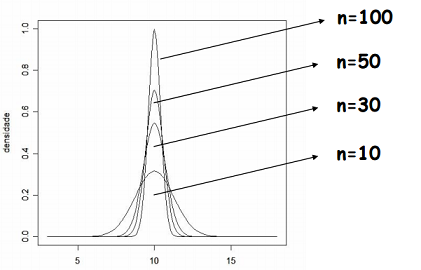
\includegraphics[scale=1.0]{EfeitoSuporte.png}	
 	\caption{Figura demonstrando o efeito de suporte para um número crescente de amostras. O aumento do número de amostras tende a concentrar a  função de densidade de probabilidade entorno do valor médio }
 	\label{Efeito_Suporte}
\end{figure}

\subsection{Teorema do limite Central}

Um dos maiores motivos da grande utilização da distribuição normal advém da lei dos grandes números. Certos procedimentos estatísticos são facilitados quando consideramos a convergência de sequências das variáveis com o aumento do número de amostras.  

Se uma variável aleatória X puder sr representada pela soma de n variáveis aleatórias independentes, então para um quantidade grande de elementos teremos uma distribuição aproximadamente normal.

Esta propriedade é aceita para qualquer distribuição de probabilidades a priori. Logo temos 

\begin{equation}
	Z_{n} = \frac{S_{n}-E(S_{n})}{\sqrt{Var(S_{n})}}
\end{equation}

Em que $S_{n}$ é a soma de variáveis aleatórias independentes. Essa distribuição se aproxima da gaussiana padronizada a medida que o número de amostras aumenta. 


\subsubsection{Teste de hipóteses}


Uma hipótese é uma suposição acerca de um dado experimento. Além dos métodos de estimação de parâmetros  estamos interessados em tomar decisões que concernem a distribuição de probabilidade daquele valor. Não rejeitar ou rejeitar uma hipótese dependerá da realidade física da estimativa concretizada pela observação das amostras. No entanto, a não rejeição, significa não haver elementos suficientes para averiguar esta possibilidade. A decisão, na verdade, sobre a hipótese não existe. Por uma questão científica, o teste de hipótese é uma ferramenta eliminatória e nunca decisiva, mesmo que em prática se adote a aceitação daquela hipótese para uma dada probabilidade.

Por tratar-se de uma inferência a respeito de uma variável aleatória, o critério de decisão está sempre associado a escolha de um nível de significância $\alpha$, que corresponde a probabilidade de rejeição da hipótese estabelecida, enquanto $(1-\alpha)$ corresponde ao intervalo de segurança, ou a probabilidade da não rejeição da hipótese nula.   

Para um teste de hipóteses geralmente definimos duas alternativas possíveis, uma hipótese nula que queremos anular e uma hipótese alternativa, que guarda outra possibilidade de ocorrência. Considere o problema em uma mineração em que se o valor médio de uma dada impureza no depósito for maior que que 5g/ton o depósito é considerado inviável. Neste caso uma distribuição gaussiana foi ajustada a partir dos dados de amostragem. 

$\left\{\begin{matrix}

 	H_{0} = \mu <  5g/ton \\ 
 	H_{1} = \mu \geqslant 5g/ton
 	
\end{matrix}\right.$

A figura \eqref{Thipotese} demonstra a situação exemplificada.

\begin{figure}[H]
  	\centering
  	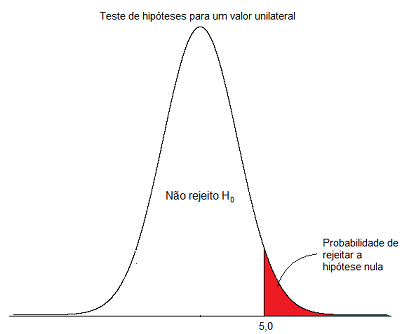
\includegraphics[scale=0.6]{Thipotese.png}	
  	\caption{Teste de hipóteses para o problema indicado. Área vermelha demonstra a probabilidade de que o valor médio da impureza no depósito exceder a 5g/ton  }
  	\label{Thipotese}
\end{figure}


Este valor demonstrado pela área vermelha também é chamado de valor p e demonstra a probabilidade calculada de se rejeitar a hipótese nula. O valor p é comparado com os limites estabelecidos pelo nível de confiabilidade. O procedimento do teste de hipóteses em geral leva aos seguinte procedimentos:

\begin{itemize}
	\item Definir a hipótese nula e alternativa do problema
	\item Definir um nível de confiabilidade para o problema
	\item Definir a estatística de teste (valor médio, variância, proporção)
	\item Definir a função de densidade de probabilidade para aquela estatística.
	\item Calcular o valor p, ou a probabilidade de se rejeitar a hipótese nula para a função de densidade de probabilidade do item anterior.
	\item Comparar o valor p com o nível de significância estabelecido
	\item Determinar se 
\end{itemize} 


\subsubsection{Ajustando uma função de densidade de probabilidade a partir de dados}

Após realizado o histograma e a estatística descritiva dos dados pode-se ajustar uma função de densidade de probabilidades. A partir de um teste de hipóteses podemos verificar a aderência do modelo. A ferramenta mais simples para se fazer isso é sem dúvida o gráfico de probabilidade. 

\begin{figure}[H]
  	\centering
  	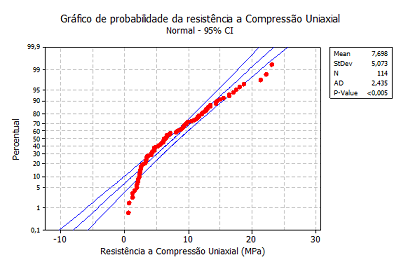
\includegraphics[scale=1.0]{Grafico_probabilidade.png}	
  	\caption{Figura demonstrando o gráfico de probabilidade da resistência a compressão uniaxial para uma distribuição de densidade de probabilidade gaussiana com intervalo de confiança de 95\% }
  	\label{Grafico_probabilidade}
\end{figure}

Note na figura que os pontos estão fora da curva azul em sua maioria. Além disso o valor-p do teste de hipóteses demonstra um valor abaixo de 0.005, que geralmente é o valor admssível para descartar a hipótese nula, que neste caso é de que a variável aleatória não assume comportamento gaussiano.  

\section{Exercícios}

\begin{itemize}
	\item Considere o conjunto de amostras com teores de ferro contendo unicamente hematita $Fe_{2}O_{3}$ e sílica $SiO_{3}$. Os valores são $\left(45,69,80,35,56,78\right)\%$. Determine os valores outliers do problema considerando a massa atômica do ferro igual 56g/mol e do oxigênio igual a 16g/mol. Resp.: 80\% e 78\%
	\item Considere o conjunto de amostras com teores $\left(2.4,5.0,7.6,4.3,2.7,8.9\right)$ g/ton todos com o mesmo suporte. Encontre o valor da média, da variância, do desvio padrão do conjunto de amostras. Resp.: $\bar{x}= 5.7$ ,$s^2 = 5.06$ , $s = 2.25$
	\item Um geólogo precisa decidir entre duas metodologias de amostragem para um dado elemento de pesquisa. Entre elas temos a sonda diamantada e o pó de perfuratriz. As incertezas do custo da pesquisa estão diretamente relacionadas com a variabilidade da recuperação, desejando o método com o menor risco associado . Para isso mediu-se a recuperação dos testemunhos e do pó retirado pela máquina. A recuperação dos testemunhos fora de 90\% com um desvio padrão de 30\%, enquanto a do pó foi de 70\% com uma variação de 20\%. Deseja-se saber qual método utilizar. Resp.: Pó de perfuratriz << CV
	\item 
	
	 
\end{itemize} 
